

\documentclass{article}
\usepackage{Sweave}

\title { Latex/Sweave Incrementally}
\author { Matt Settles }
\begin {document}
\maketitle

\section{Basic Sweave Example with figure}
This is a basic example with a figure

\begin{Schunk}
\begin{Sinput}
> options(width=40)
> x <- 1:10
> y <- x^2
> y
\end{Sinput}
\begin{Soutput}
 [1]   1   4   9  16  25  36  49  64  81
[10] 100
\end{Soutput}
\end{Schunk}

\begin{center}
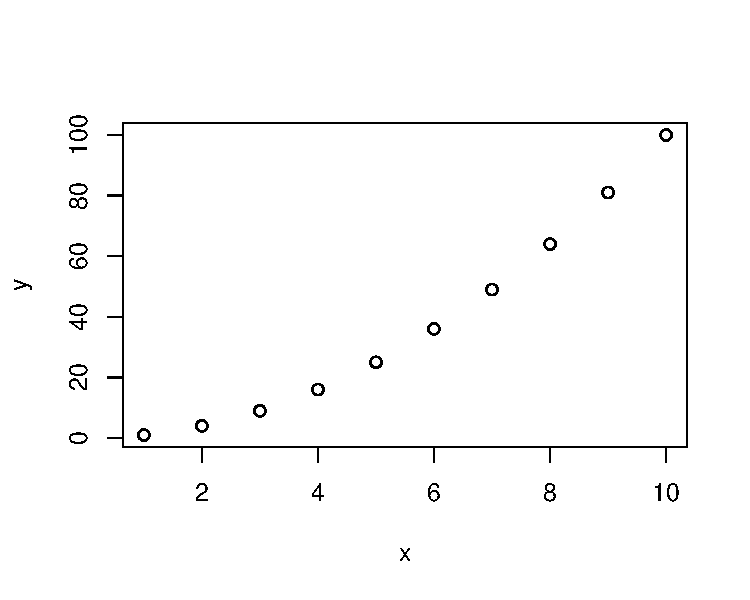
\includegraphics{Sweave-002}
\end{center}

\section{making tables in sweave}
A data frame of sequencing quality characters


\begin{center}
% latex table generated in R 2.14.1 by xtable 1.6-0 package
% Wed Feb 29 08:46:15 2012
\begin{table}[tbp]
\begin{center}
\caption{Quality Scores by value}
\label{table:qual}
\begin{tabular}{rll}
  \hline
numeric & phred & illumina64 \\ 
  \hline
  0 & ! &  \\ 
    1 & " &  \\ 
    2 & \# & B \\ 
    3 & \$ & C \\ 
    4 & \% & D \\ 
    5 & \& & E \\ 
    6 & ' & F \\ 
    7 & ( & G \\ 
    8 & ) & H \\ 
    9 & * & I \\ 
   10 & + & J \\ 
   11 & , & K \\ 
   12 & - & L \\ 
   13 & . & M \\ 
   14 & / & N \\ 
   15 & 0 & O \\ 
   16 & 1 & P \\ 
   17 & 2 & Q \\ 
   18 & 3 & R \\ 
   19 & 4 & S \\ 
   20 & 5 & T \\ 
   21 & 6 & U \\ 
   22 & 7 & V \\ 
   23 & 8 & W \\ 
   24 & 9 & X \\ 
   25 & : & Y \\ 
   26 & ; & Z \\ 
   27 & $<$ & [ \\ 
   28 & = & $\backslash$ \\ 
   29 & $>$ & ] \\ 
   30 & ? & \verb|^| \\ 
   31 & @ & \_ \\ 
   32 & A & ` \\ 
   33 & B & a \\ 
   34 & C & b \\ 
   35 & D & c \\ 
   36 & E & d \\ 
   37 & F & e \\ 
   38 & G & f \\ 
   39 & H & g \\ 
   40 & I & h \\ 
   41 &  & i \\ 
   \hline
\end{tabular}
\end{center}
\end{table}
\end{center}
\end{document}
